\section{Organisation d'un projet}

\begin{frame}
	\begin{center}
		\huge
		Organisation d'un projet
	\end{center}
\end{frame}

\subsection{Les modules} %%%%%%%%%%%%%%%%%%%%%%%%%%%%%%%%%%%%%%%%%%%%%%%%%%%%%%
\begin{frame}
	\frametitle{Principe des modules}
	\begin{center}
		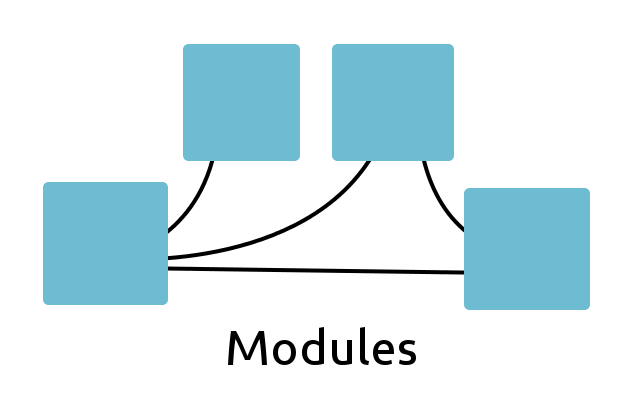
\includegraphics[width=9cm]{pics/modules.png}
	\end{center}
\end{frame}

\begin{frame}[fragile]
	\frametitle{Modules}
	\framesubtitle{Utilisation de fonctions d'un module}
	\begin{block}{Avec \textit{open}}
		\begin{lstlisting}
  open List

  length 
    (1::3::3::7::[])
		\end{lstlisting}
	\end{block}
	\begin{block}{Sans \textit{open}}
		\begin{lstlisting}
  List.length 
    (1::3::3::7::[])
		\end{lstlisting}
	\end{block}
\end{frame}

\begin{frame}
	\frametitle{Modules}
	\framesubtitle{Une façon de créer un module : Un fichier}
	\begin{columns}[t]
		\begin{column}{3cm}
			\begin{block}{Fichiers Source}
				main.ml\\
				processing.ml\\
				rotation.ml\\
				cutting.ml\\
				recognition.ml
			\end{block}
		\end{column}
		\begin{column}{3cm}
			\begin{block}{Fichiers Interface}
				processing.mli\\
				rotation.mli\\
				cutting.mli\\
				recognition.mli
			\end{block}
		\end{column}
	\end{columns}
\end{frame}

\begin{frame}[fragile]
	\frametitle{Les fichiers interface}
	\begin{block}{someFunctions.ml}
		\begin{lstlisting}
  let add a b = a + b
  let addf a b = a +. b
  let sub a b = a - b
  let subf a b = a -. b
		\end{lstlisting}
	\end{block}
	\begin{block}{someFunctions.mli}
		\begin{lstlisting}
  val add :  int -> int -> int
  val addf : float -> float -> float
  val sub : int -> int -> int
  val subf : float -> float -> float
		\end{lstlisting}
	\end{block}
\end{frame}

\begin{frame}[fragile]
	\frametitle{Les fichiers interface}
	\framesubtitle{Syntaxe d'un fichier interface 1/3}
	\lstset{basicstyle=\small}
	\begin{lstlisting}
val f : int -> int -> int

exception badSurface of (int -> int) * int

type card =
| Ace
| Number of int
| Head of HeadCard

type coloredPoint = {
  pos : int * int;
  mutable color;
}
	\end{lstlisting}
\end{frame}

\begin{frame}[fragile]
	\frametitle{Les fichiers interface}
	\framesubtitle{Syntaxe d'un fichier interface 2/3}
	\lstset{basicstyle=\small}
	\begin{lstlisting}
(* Simple class *)
class counter :
  object
    val mutable i : int
    method getCounts : unit -> int
  end

(* Class with initialization parameter *)
class point :
  int * int -> 
    object
      val pos : int * int
      method printCoord : unit -> unit
    end
	\end{lstlisting}
\end{frame}

\begin{frame}[fragile]
	\frametitle{Les fichiers interface}
	\framesubtitle{Syntaxe d'un fichier interface 3/3}
	\lstset{basicstyle=\small}
	\begin{lstlisting}
(* Class with type parameter *)
class ['a] storage = 
  object 
    val mutable data : 'a list
    method addData : 'a -> unit 
  end
	\end{lstlisting}
\end{frame}

\subsection{La compilation avec ocamlbuild} %%%%%%%%%%%%%%%%%%%%%%%%%%%%%%%%%%%
\begin{frame}[fragile]
	\frametitle{Les differents modes d'exécution}
	\huge
	\begin{itemize}
		\item ocaml : Interprétation directe 
		\item ocamlc : Compilation byte-code
		\item ocamlopt : Compilation native
	\end{itemize}
	\normalsize
\end{frame}

\begin{frame}
	\frametitle{Le travail d'un Makefile}
	\begin{center}
		\begin{itemize}
			\item Lister les fichiers sources
			\item Trouver/Indiquer les chemins d'accès des bibliothèques
			\item Indiquer les outils de compilation
			\item Générer les fichiers correspondant à chaque étape de la compilation
			\item Gérer les dépendances entre les modules
		\end{itemize}
	\end{center}
\end{frame}

\begin{frame}[fragile]
	\frametitle{ocamlbuild}
	\begin{block}{Commande générique}
		\begin{lstlisting}
  42sh$ ocamlbuild -use-ocamlfind\
    -pkgs [library] [mainFile].[byte/native]
		\end{lstlisting}
	\end{block}
	\begin{block}{Exemple}
		\begin{lstlisting}
  42sh$ ocamlbuild -use-ocamlfind -pkgs\
    lua,expat,sdl,sdl.sdlimage,sdl.sdlttf,str\
    main.native
		\end{lstlisting}
	\end{block}
\end{frame}

\subsection{Faire de la documentation} %%%%%%%%%%%%%%%%%%%%%%%%%%%%%%%%%%%%%%%%
\begin{frame}
	\frametitle{La documentation}
	\begin{center}
		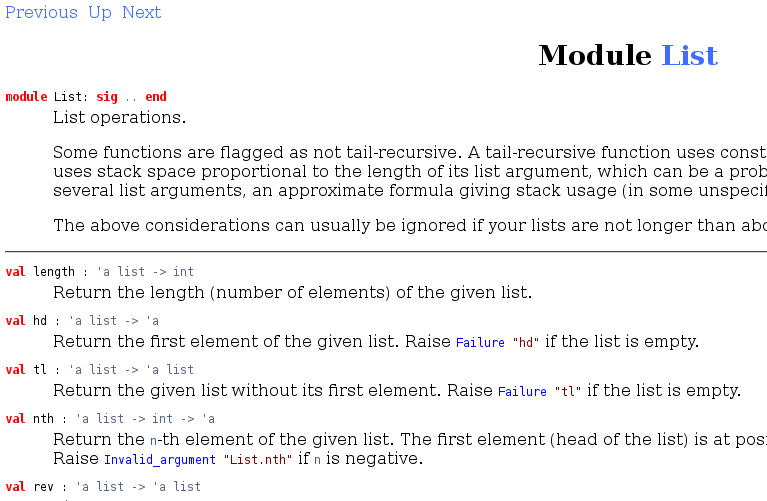
\includegraphics[width=10cm]{pics/doc.png}
	\end{center}
\end{frame}

\begin{frame}[fragile]
	\frametitle{ocamldoc via ocamlbuild}
	\begin{block}{previousEx.odocl}
		\begin{lstlisting}
  Main
  Processing
  Rotation
  Cutting
  Recongnition
		\end{lstlisting}
	\end{block}
	\begin{block}{Commande}
		\begin{lstlisting}
  # ocamlbuild previousEx.docdir/index.html
		\end{lstlisting}
	\end{block}
\end{frame}

\begin{frame}[fragile]
	\frametitle{Les commentaires de ocamldoc 1/2}
	\lstset{basicstyle=\scriptsize}	
	\begin{lstlisting}
(** The first special comment of the file is the 
    comment associated with the whole module.*)

(******************************************************)
(** Comments like the one above, with more than two 
    asterisks, are ignored. *)

(** The comment for function f. *)
val f : int -> int -> int
(** The continuation of the comment for function f. *)


(** Comment for type weather  *)
type weather =
| Rain of int (** The comment for construtor Rain *)
| Sun (** The comment for constructor Sun *)
	\end{lstlisting}
\end{frame}

\begin{frame}[fragile]
	\frametitle{Les commentaires de ocamldoc 2/2}
	\lstset{basicstyle=\scriptsize}	
	\begin{lstlisting}
(** The comment for class my_class *)
class my_class :
  object
    (** A comment to describe inheritance from cl *)
    inherit cl

    (** The comment for attribute tutu *)
    val mutable tutu : string

    (** The comment for attribute toto. *)
    val toto : int

    (** This comment is not attached to titi since
        there is a blank line before titi, but is kept
        as a comment in the class. *)

    val titi : string

    (** Comment for method toto *)
    method toto : string

    (** Comment for method m *)
    method m : float -> int
  end
	\end{lstlisting}
\end{frame}

